\begin{figure}[h!]
   \centering
   \begin{subfigure}[b]{0.4\textwidth}
      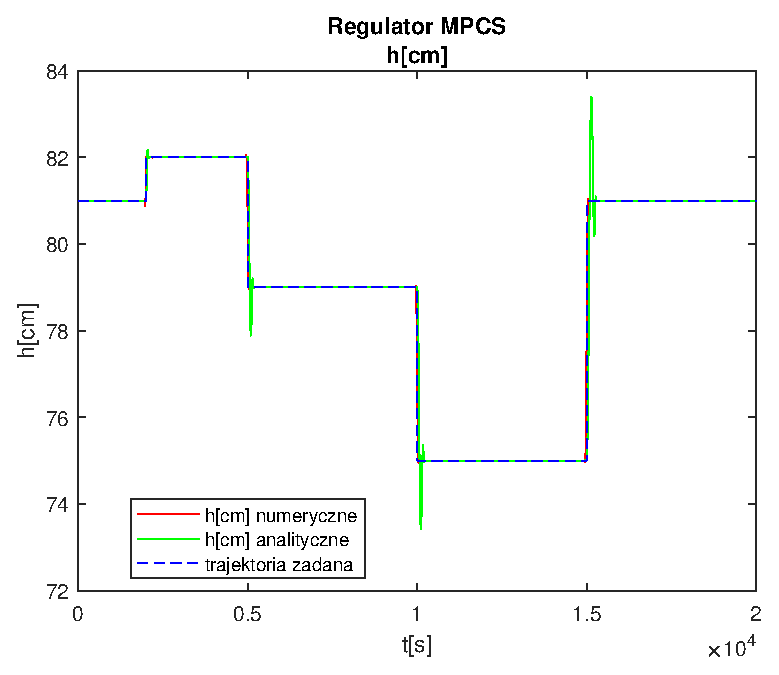
\includegraphics[width=1\linewidth]{img/MPCSnumRK/MPCSRKHN50Nu10l20.eps}
      \caption{}
      \label{fig:fig:MPCSRKN50Nu10l201}
   \end{subfigure}
       
   \begin{subfigure}[b]{0.4\textwidth}
      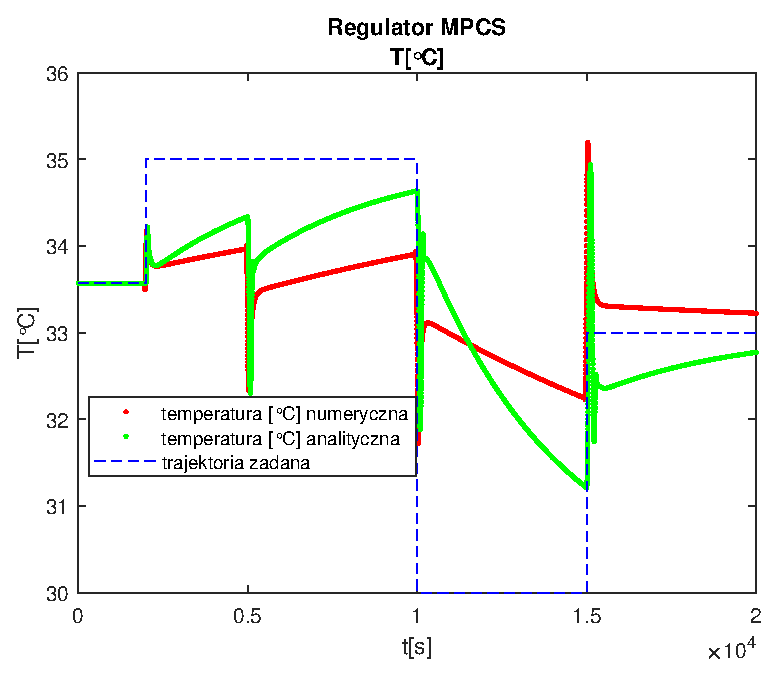
\includegraphics[width=1\linewidth]{img/MPCSnumRK/MPCSRKTN50Nu10l20.eps}
      \caption{}
      \label{fig:fig:MPCSRKN50Nu10l202}
   \end{subfigure}
       
   \begin{subfigure}[b]{0.4\textwidth}
      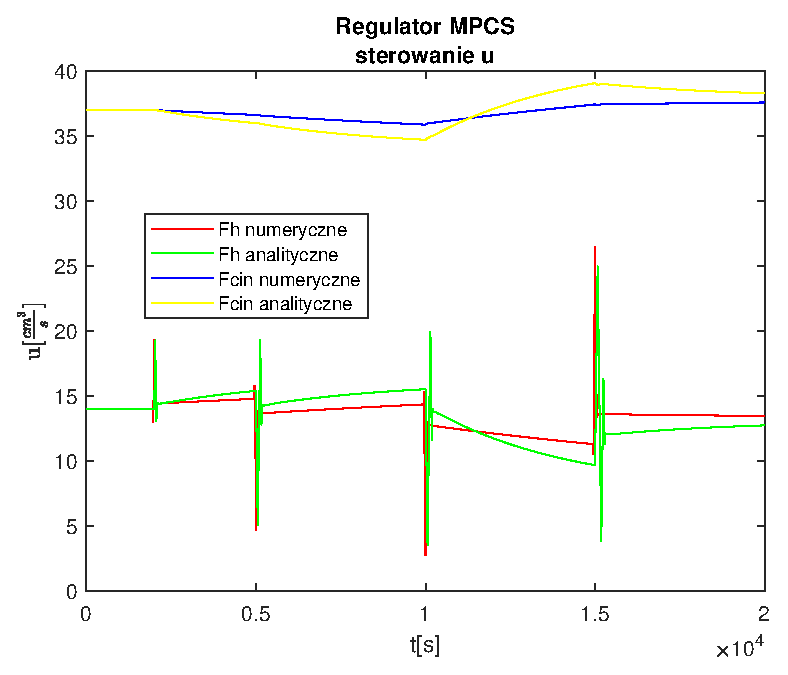
\includegraphics[width=1\linewidth]{img/MPCSnumRK/MPCSRKControlN50Nu10l20.eps}
      \caption{}
      \label{fig:fig:MPCSRKN50Nu10l203}
   \end{subfigure}
       
   \caption{Wykresy dla regulatora MPCS, obiekt nieliniowy, $N = 50$, $N_u = 10$.}
   \label{fig:MPCSRKN50Nu10l20}
\end{figure}
           
